\documentclass[a4paper, fontsize=14pt]{article}
\usepackage[T2A]{fontenc}
\usepackage{mathtools}
\usepackage[utf8]{inputenc}
\usepackage[english, russian]{babel}
\usepackage{fancyhdr}
\usepackage{graphicx}
\usepackage{gensymb}
\usepackage{floatrow}
\usepackage{titlesec}
\usepackage{lastpage}
\usepackage{float}
\usepackage{gensymb}
\usepackage{booktabs}
\usepackage{amsmath}
\usepackage{amssymb}


\pagestyle{fancy}
	\fancyhf{}
	\lhead{\hspace{1bp} Работа \textnumero 4.1.2}
	\rhead{Фирстов Сергей 878\hspace{1bp}}
	\cfoot{\textbf{}}
	\rfoot{\thepage\ \textnormal{из}\ \pageref{LastPage}}
	\renewcommand{\headrulewidth}{1pt}
	\renewcommand{\footrulewidth}{1pt}


%\addtolength{\hoffset}{-1.75cm}
%\addtolength{\textwidth}{3.5cm} 

%\addtolength{\voffset}{-1.5cm}
%\addtolength{\textheight}{3cm} 

\titleformat{\section}
    [block]{\normalfont\bfseries\large}{\rlap{\thesection}}{0em}
    {\vspace{-0.02\textwidth}\begin{minipage}[t]{.95\textwidth}}
[\end{minipage}]

\thispagestyle{fancy}

\begin{document}
\selectlanguage{russian}



\huge
\centering
\textbf{Петля гистерезиса (динамический метод)}

\raggedright
\large
\parindent=1cm
\section*{Цель работы}
Изучение петель гистерезиса ферромагнитных материалов с помощью осциллографа.
\section*{Оборудование}
Автотрансформатор, понижающий трансформатор, интегрирующая цепочка, амперметр, вольтметр, электронный осциллограф, делитель напряжения, тороидальные образцы с двумя обмотками.
\section*{Экспериментальная установка}
\begin{figure}[H]
\center
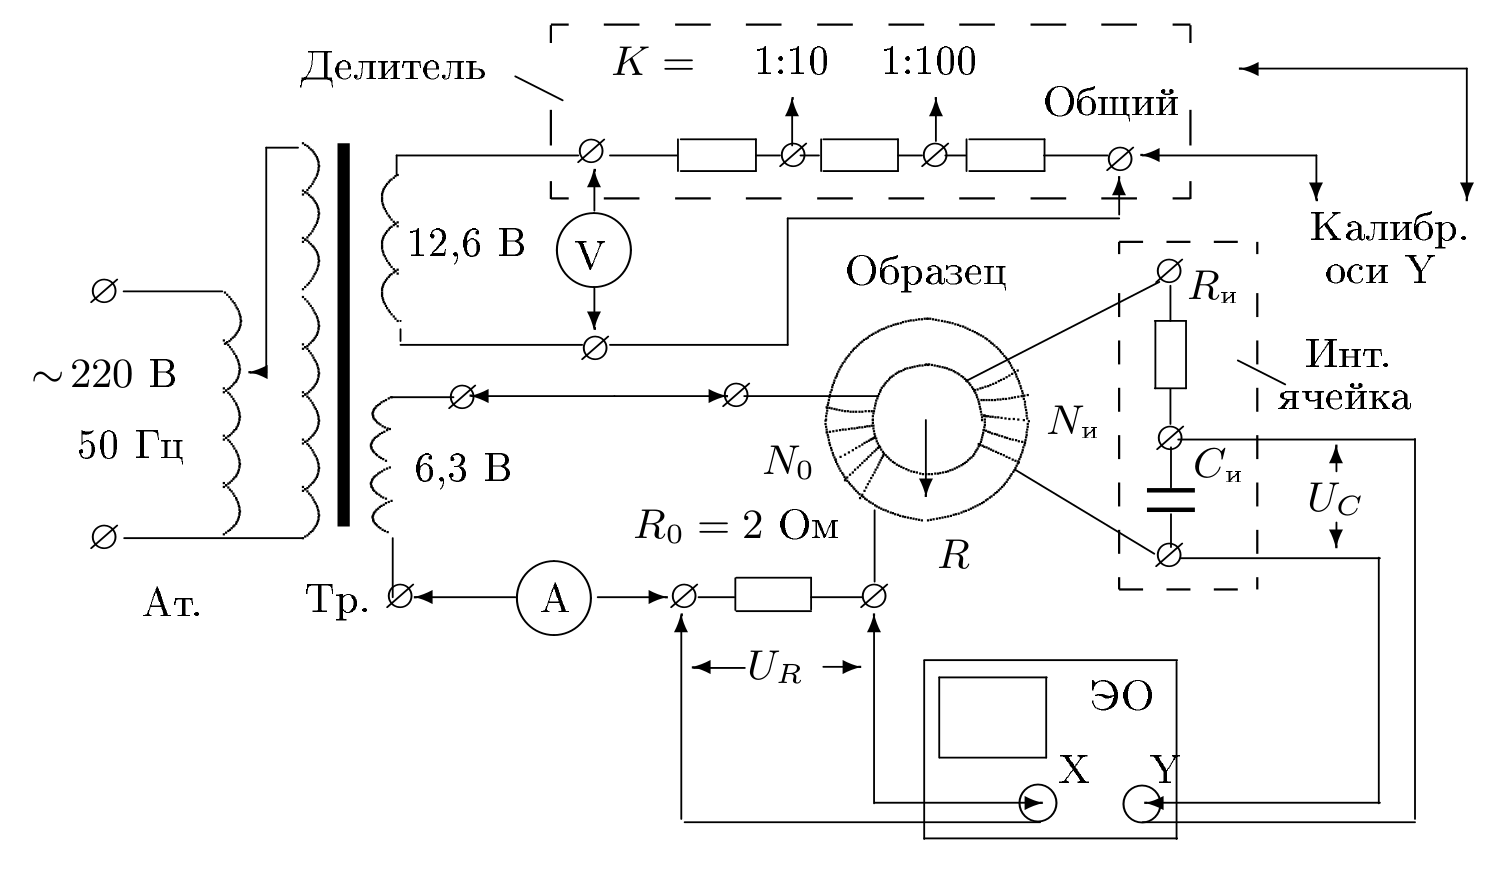
\includegraphics[scale=0.2]{ust.png}
\caption{Схема установки для исследования намагничивания образцов}
\end{figure}

\section*{Теоретическая часть}
Действующее значение переменного тока в обмотке $N_0$ измеряется амперметром $A$ (мультивольтметром GDM). Последовательно с амперметром включено сопротивление $R_0$, напряжение с которого подаётся на вход $X$ электронного осциллографа (ЭО). Это напряжение пропорционально току в обмотке $N_0$, а следовательно и напряжённости $H$ магнитного поля в образце.

Для измерения магнитной индукции $B$ с измерительной обмотки $N_\text{И}$ на вход интегрирующей $RC$-цепочки подаётся напряжение $U_\text{И} (U_\text{ВХ})$, пропорциональное производной $\dot B$, а с выхода снимается напряжение $U_C (U_\text{ВЫХ})$, пропорциональное величине $B$, и подаётся на вход $Y$ осциллографа.

Замкнутая кривая, аозникающая на экране, воспроизводит в некотором масштабе (различном для осей $X$ и $Y$) петлю гистерезиса. Чтобы придать этой кривой количественный смысл, необходимо установить масштабы изображения, т.е. провести калибровку каналов $X$ и $Y$ ЭО. Для этого, во-первых, надо узнать, каким напряжениям (или токам) соответствуют амплитуды сигналов, видимых на экране, и во-вторых --- каким значениям $B$ и $H$ соответствуют эти напряжения (или токи).

Исследуемый сигнал подаётся на вход $X$; длина $2x$ горизонтальной черты, наблюдаемой на экране, характеризует удвоенную амплитуду сигнала.

Если известна чувствительность усилителя $K_X$ в вольтах на деление шкалы экрана, то удвоенная амплитуда напряжения определяется произведением
\[
	2 U_{X, 0} = 2x \cdot K_X.
\]
Напряжение, подаваемое на ось $Y$, измеряется аналогично.

Калибровку осей осциллографа ($K_X$ и $K_Y$) можно использовать для построения кривой гистерезиса в координатах $B$ и $H$, зная величину сопротивления $R_0$ с которого снимается сигнал, можно определить чувствительность канала по току $K_{XI} = K_X / R_0 $ [А/дел]; затем, используя формулу, определить цену деления шкалы в А/м. Таким же образом определяется цена деления оси $Y$:
\[
	m_x = \frac{2R_0 \sqrt{2} I_\text{ЭФ}}{2x}\ \frac{\text{В}}{\text{дел}}.
\]
\[
	m_y = \frac{2 \sqrt{2} K U_\text{ЭФ}}{2y}\ \frac{B}{\text{дел}}.1
\]
\section*{Обработка результатов экспериментов}
Рассчитаeм значения $m_X$ и $m_Y$ и сравним с величинами $K_X$ и $K_Y$, использованных при калибровке:
\[
	I_\text{ЭФ} = 1.74\ A; 2x = 9.6\ \text{дел} \Rightarrow m_x = 1.025\ \frac{\text{В}}{\text{дел}}, K_X = 1\ B
\]
\[
	U_\text{ЭФ} = 128.9\ \text{мВ}; 2y = 7.5\ \text{дел}  \Rightarrow m_y = 48.6\ \frac{\text{мВ}}{\text{дел}}, K_Y = 50\ \text{мВ}
\]
Рассчитаем постоянную времени $\tau = RC$, рассчитанную по формуле $\tau = U_\text{ВХ} / (\Omega U_\text{ВЫХ})$, с рассчётом через параметры $R_\text{И}$ и $C_\text{И}$, указанные на установке:
\[
	U_\text{ВХ} = 7.2\ B; U_\text{ВЫХ} = 0.057\ B \Rightarrow \tau = 0.402 c
\]
\[
	R_\text{И} = 20 \cdot 10^3\ \text{Ом}; C_\text{И} = 20 \cdot 10^{-6} \Rightarrow \tau = 0.4 c
\]
\[
	R = 20 \cdot 10^3 \ \text{Ом} \gg \frac{1}{\Omega C} = 159\ c
\]
С достаточной точностью выполняется условие $R \gg 1 / (\Omega C)$.

Для каждого образца рассчитаем цену деления ЭО: для оси $X$ --- в А/м на одно деление, для оси $Y$ --- в Тс на одно деление. Рассчитаем коэрцитивную силу $H_c$ и индукцию насыщения $B_S$ для каждого образца, оценим максимальное значение дифференциальной магнитной проницаемости $\mu_\text{диф}$ по начальным кривым намагничивания:

\textbf{Пермаллой (Fe - Ni)}
\[
	N_0 = 20\ \text{в.};\ N_\text{И} = 300\ \text{в.};\ S = 0.76\ \text{см}^2;\ 2 \pi R = 13.3\ \text{см}
\]
\begin{table}[H]
	\centering
	\begin{tabular}{|c|c|c|} \hline
		$I,\ A$ &  $x,\ \text{дел}$ & $y,\ \text{дел}$ \\\hline
		0.129 & 4.1 & 2.7 \\\hline
		0.111 & 3 & 1.7 \\\hline
		0.96 & 2.5 & 1.3 \\\hline
		0.85 & 2.2 & 1.0 \\\hline
		0.67 & 1.6 & 0.6 \\\hline
	\end{tabular}	
\end{table}
\begin{figure}[H]
\center
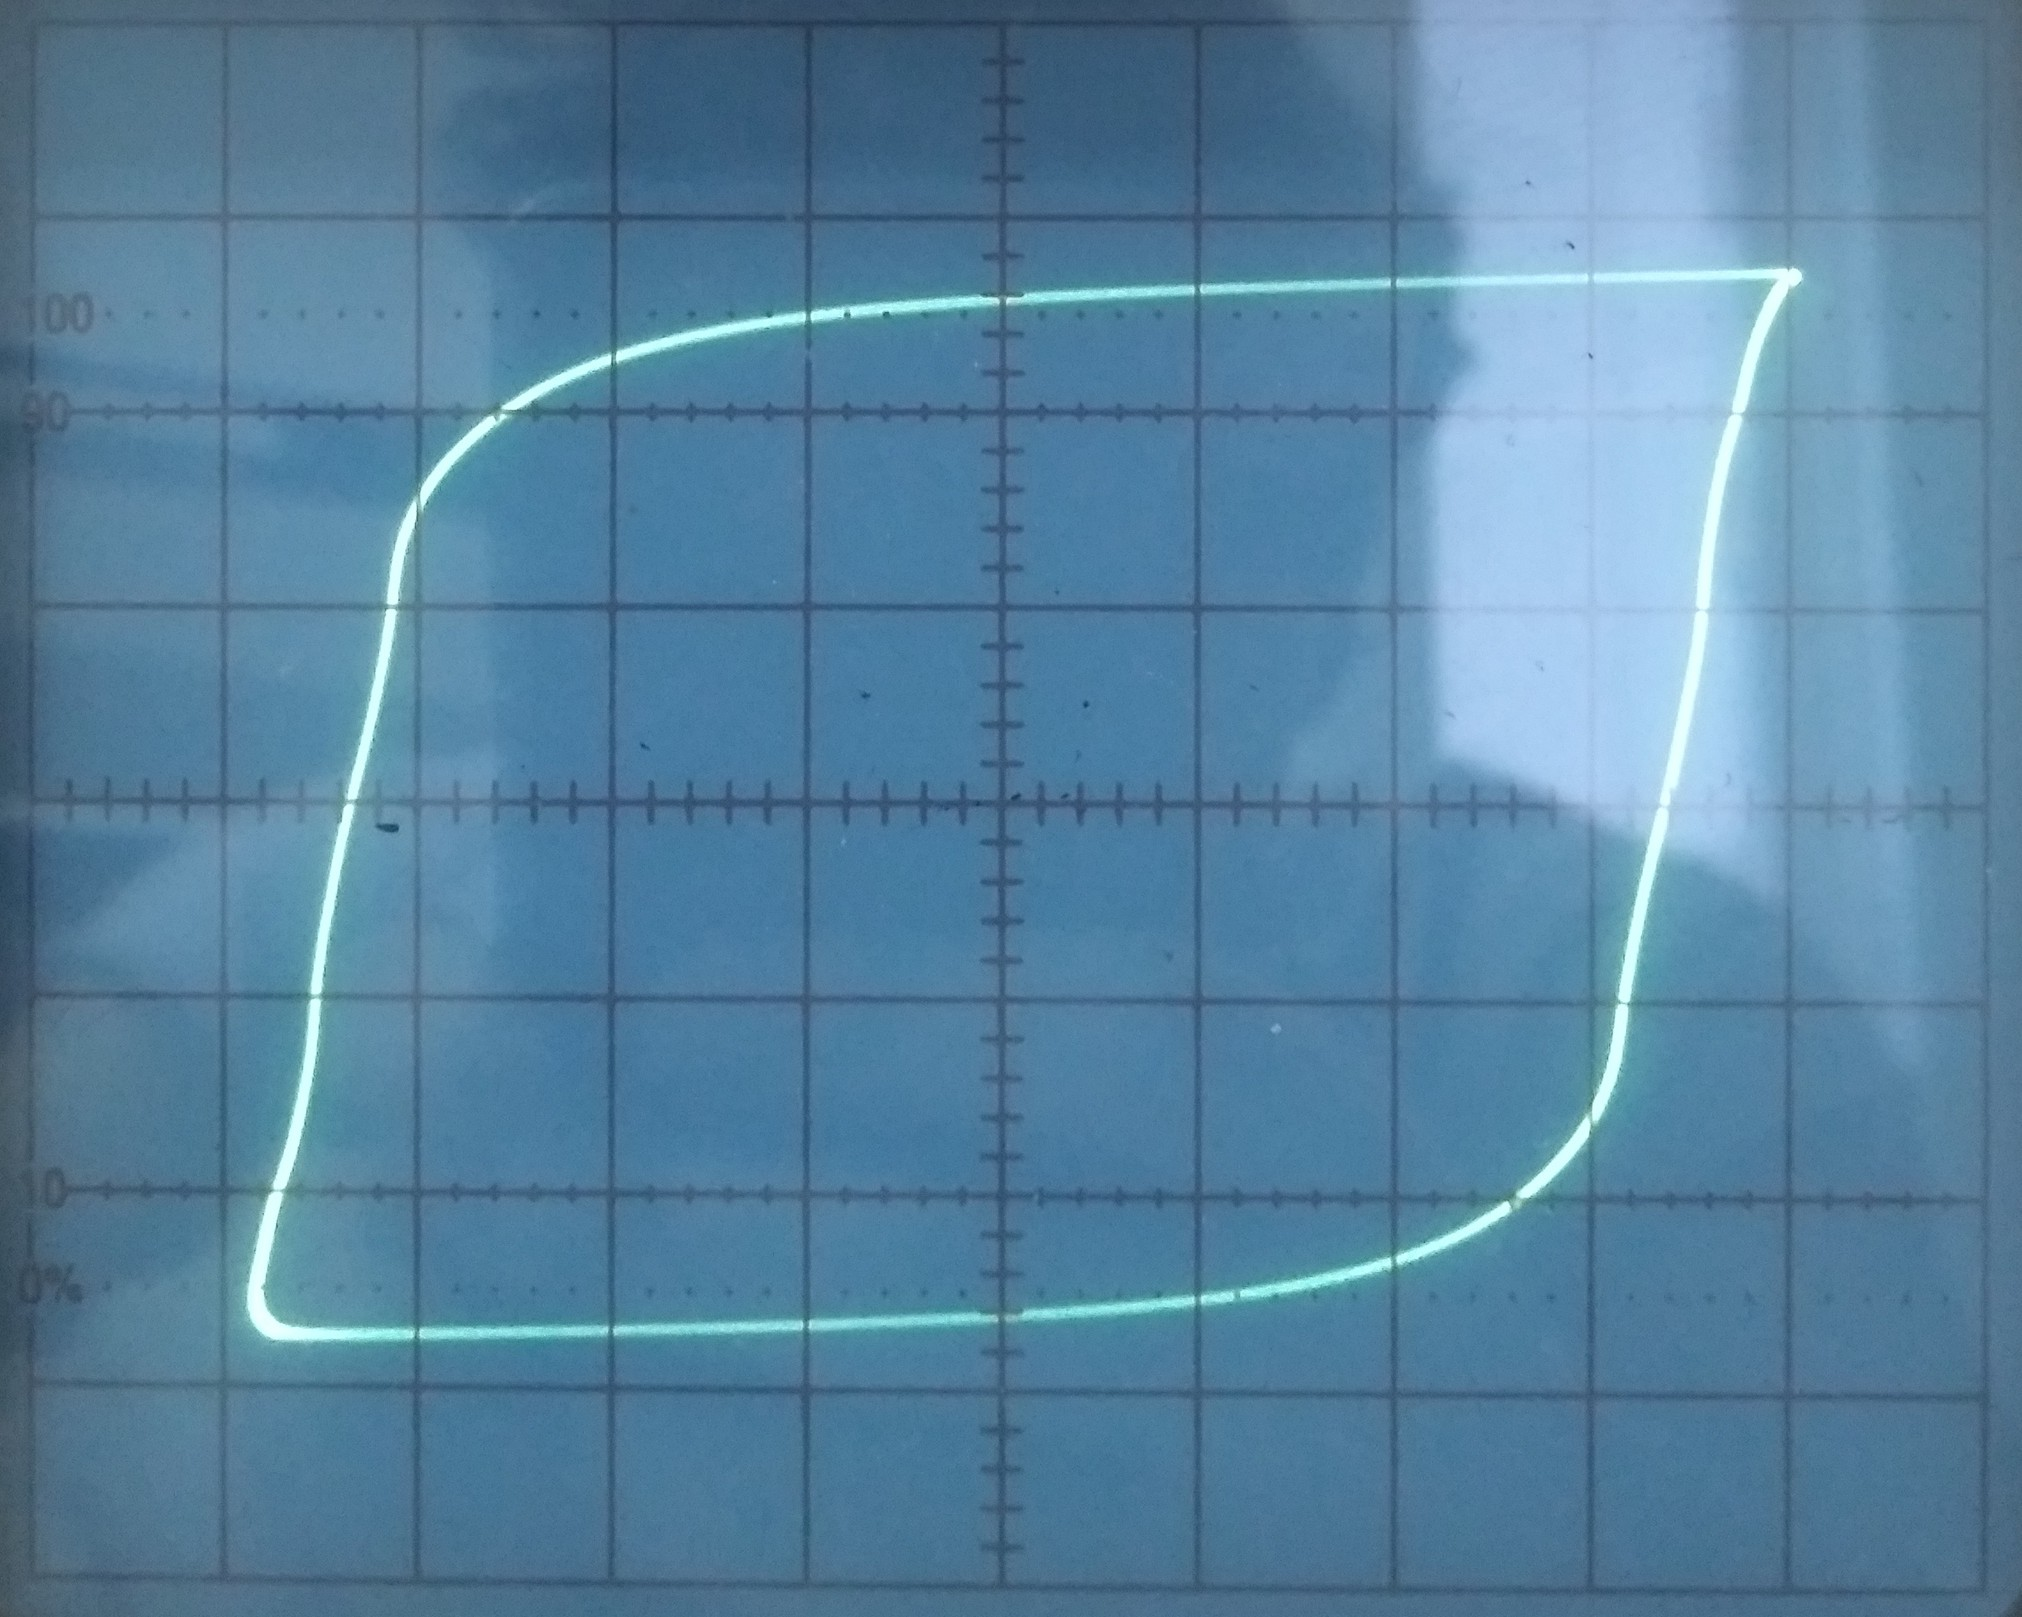
\includegraphics[scale=0.1]{per1.jpg}
\caption{Максимальная петля гистерезиса для пермаллоя}
\end{figure}
\begin{figure}[H]
\center
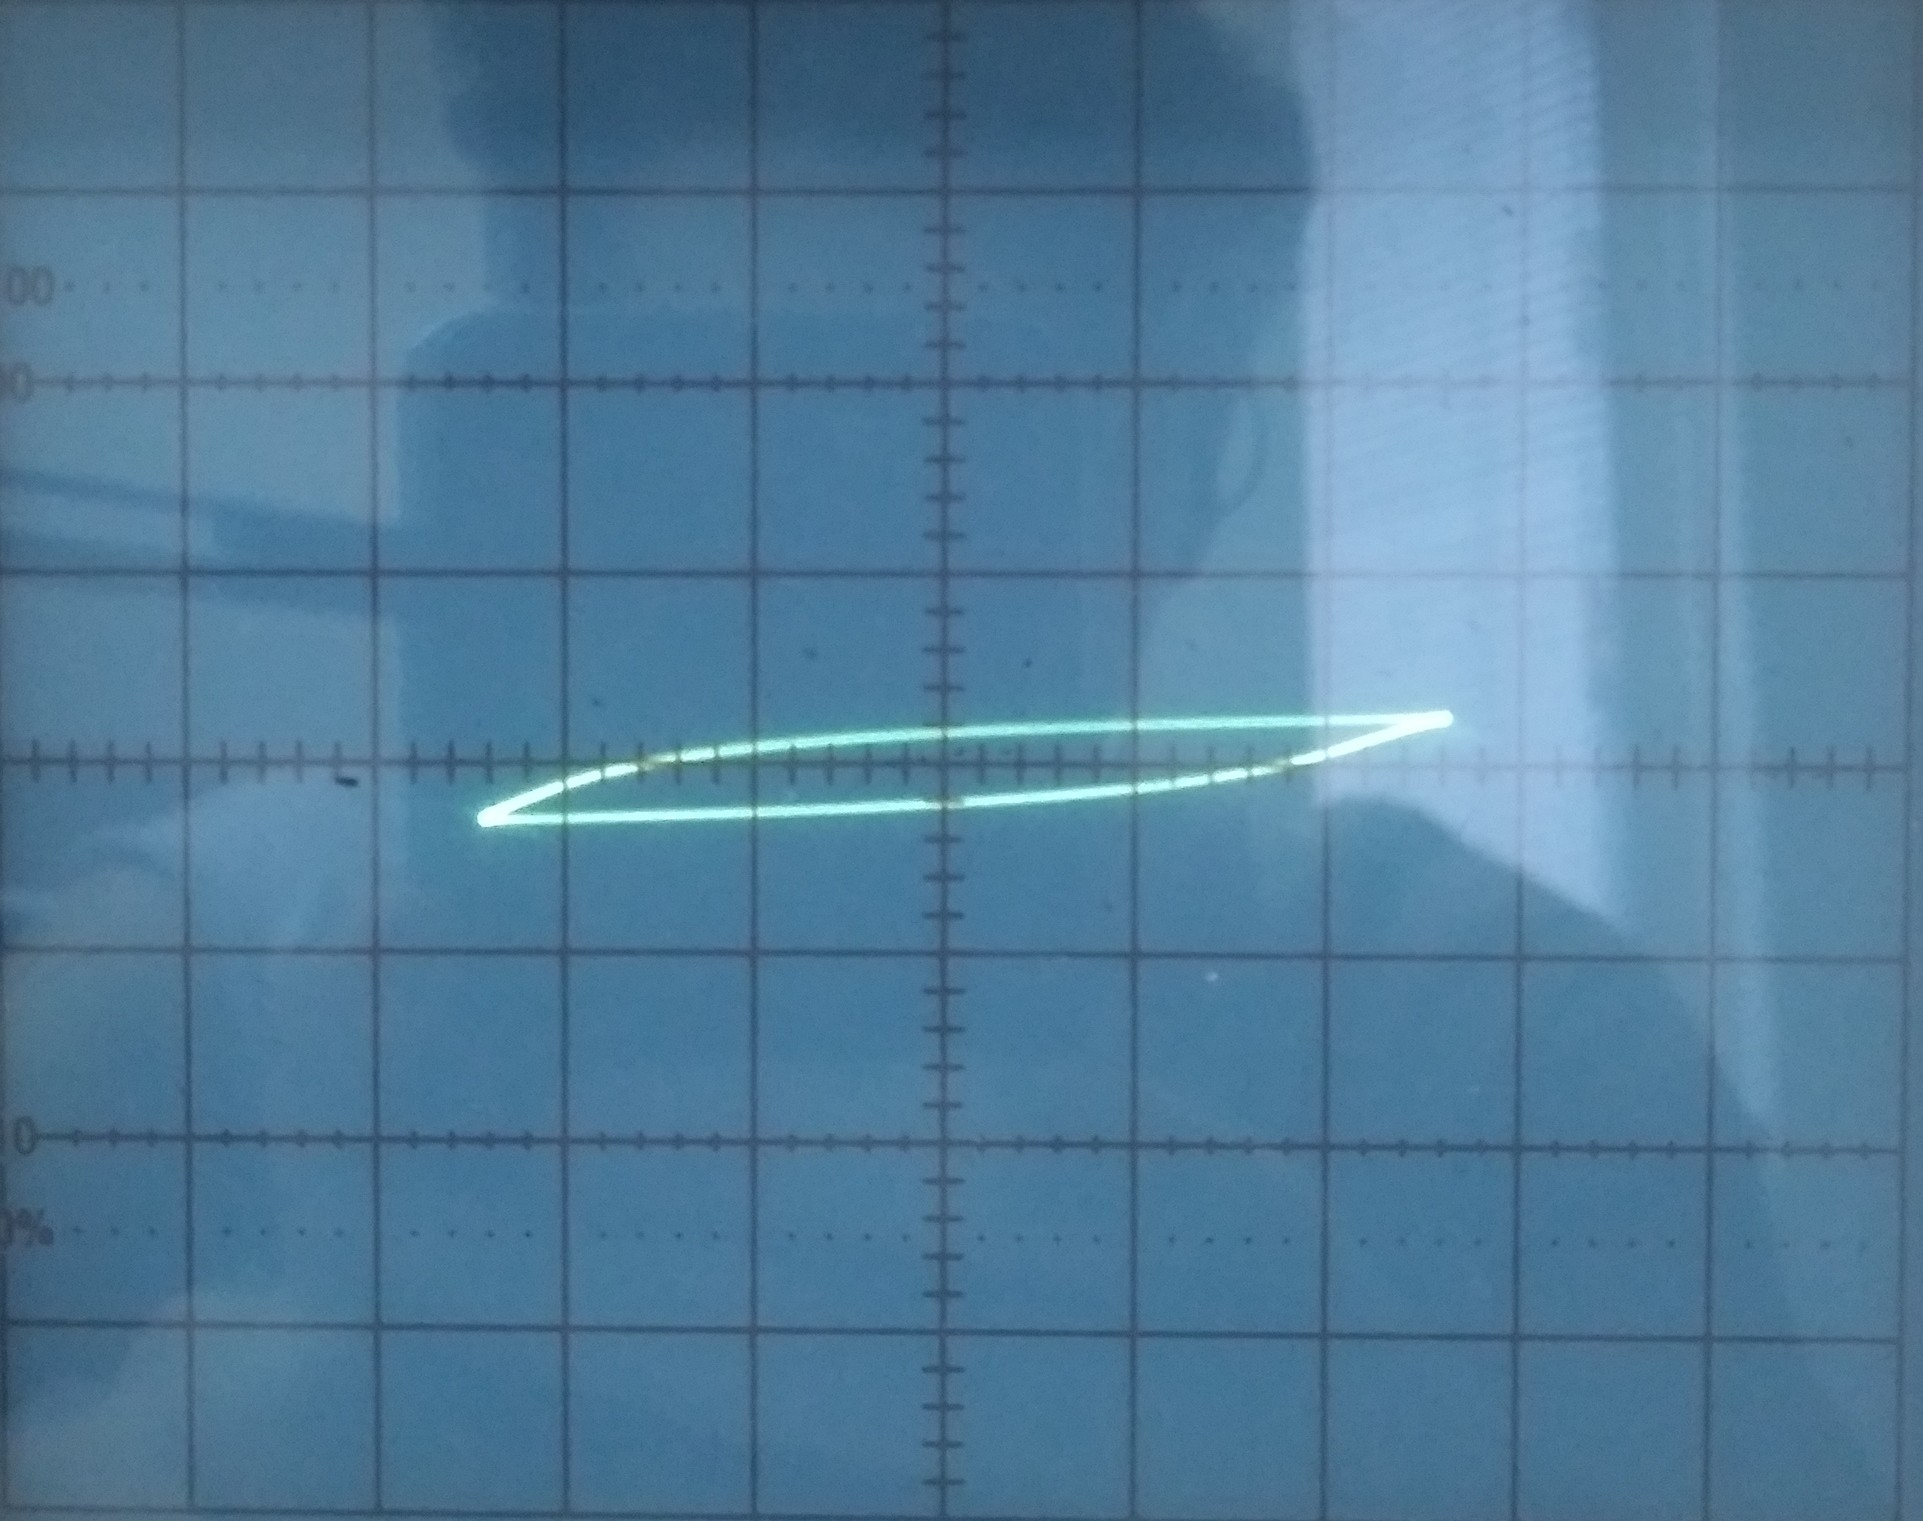
\includegraphics[scale=0.1]{per2.jpg}
\caption{Петля гистерезис1а меньшего размера для пермаллоя}
\end{figure}

\[
	K_X = 0.1\ B;\ K_Y = 50\ \text{мВ};\ I_\text{ЭФ} = 0.129 A
\]
\[
	2x(c) = 8\ \text{дел};\ 2y(s) = 5.2\ \text{дел}
\]
\[
	H = \frac{I N_0}{2 \pi R} = 7.5\ \frac{A}{\text{м}};\ H_c = 0.23\ \frac{A}{\text{м}}
\]
\[
B = \frac{R_\text{И} C_\text{И} U_\text{ВЫХ}}{S N_\text{И}} = 0.877\ \text{Тл};\ B_s = 1.4\ \text{Тл}
\]
\begin{figure}[H]
\center
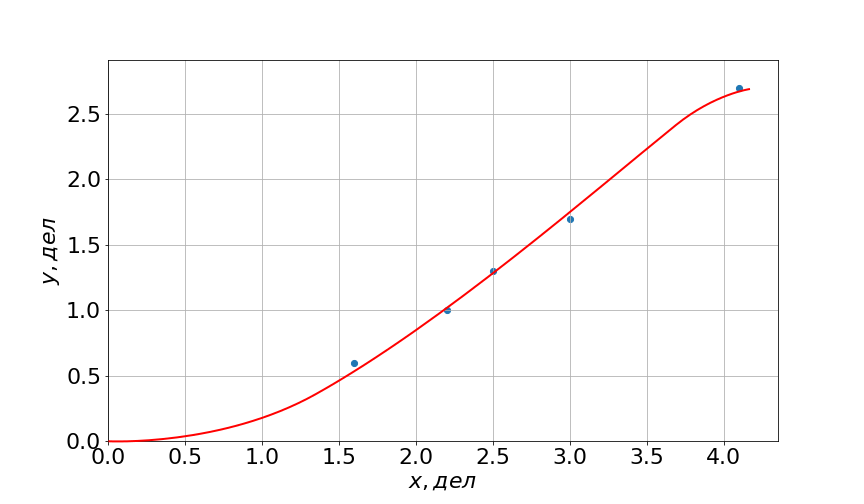
\includegraphics[scale=0.4]{11.png}

\end{figure}
\textbf{Кремнистое железо (Fe - Si)}
\[
	N_0 = 25\ \text{в.};\ N_\text{И} = 250\ \text{в.};\ S = 2.00\ \text{см}^2;\ 2 \pi R = 11.0\ \text{см}
\]
\begin{table}[H]
	\centering
	\begin{tabular}{|c|c|c|} \hline
		$I,\ A$ &  $x,\ \text{дел}$ & $y,\ \text{дел}$ \\\hline
		1.384 & 4.2 & 3.4 \\\hline
		0.986 & 2.8 & 2.7 \\\hline
		0.799 & 2.3 & 2.4 \\\hline
		0.561 & 1.6 & 2.0 \\\hline
		0.345 & 1.0 & 1.4 \\\hline
	\end{tabular}	
\end{table}

\begin{figure}[H]
\center
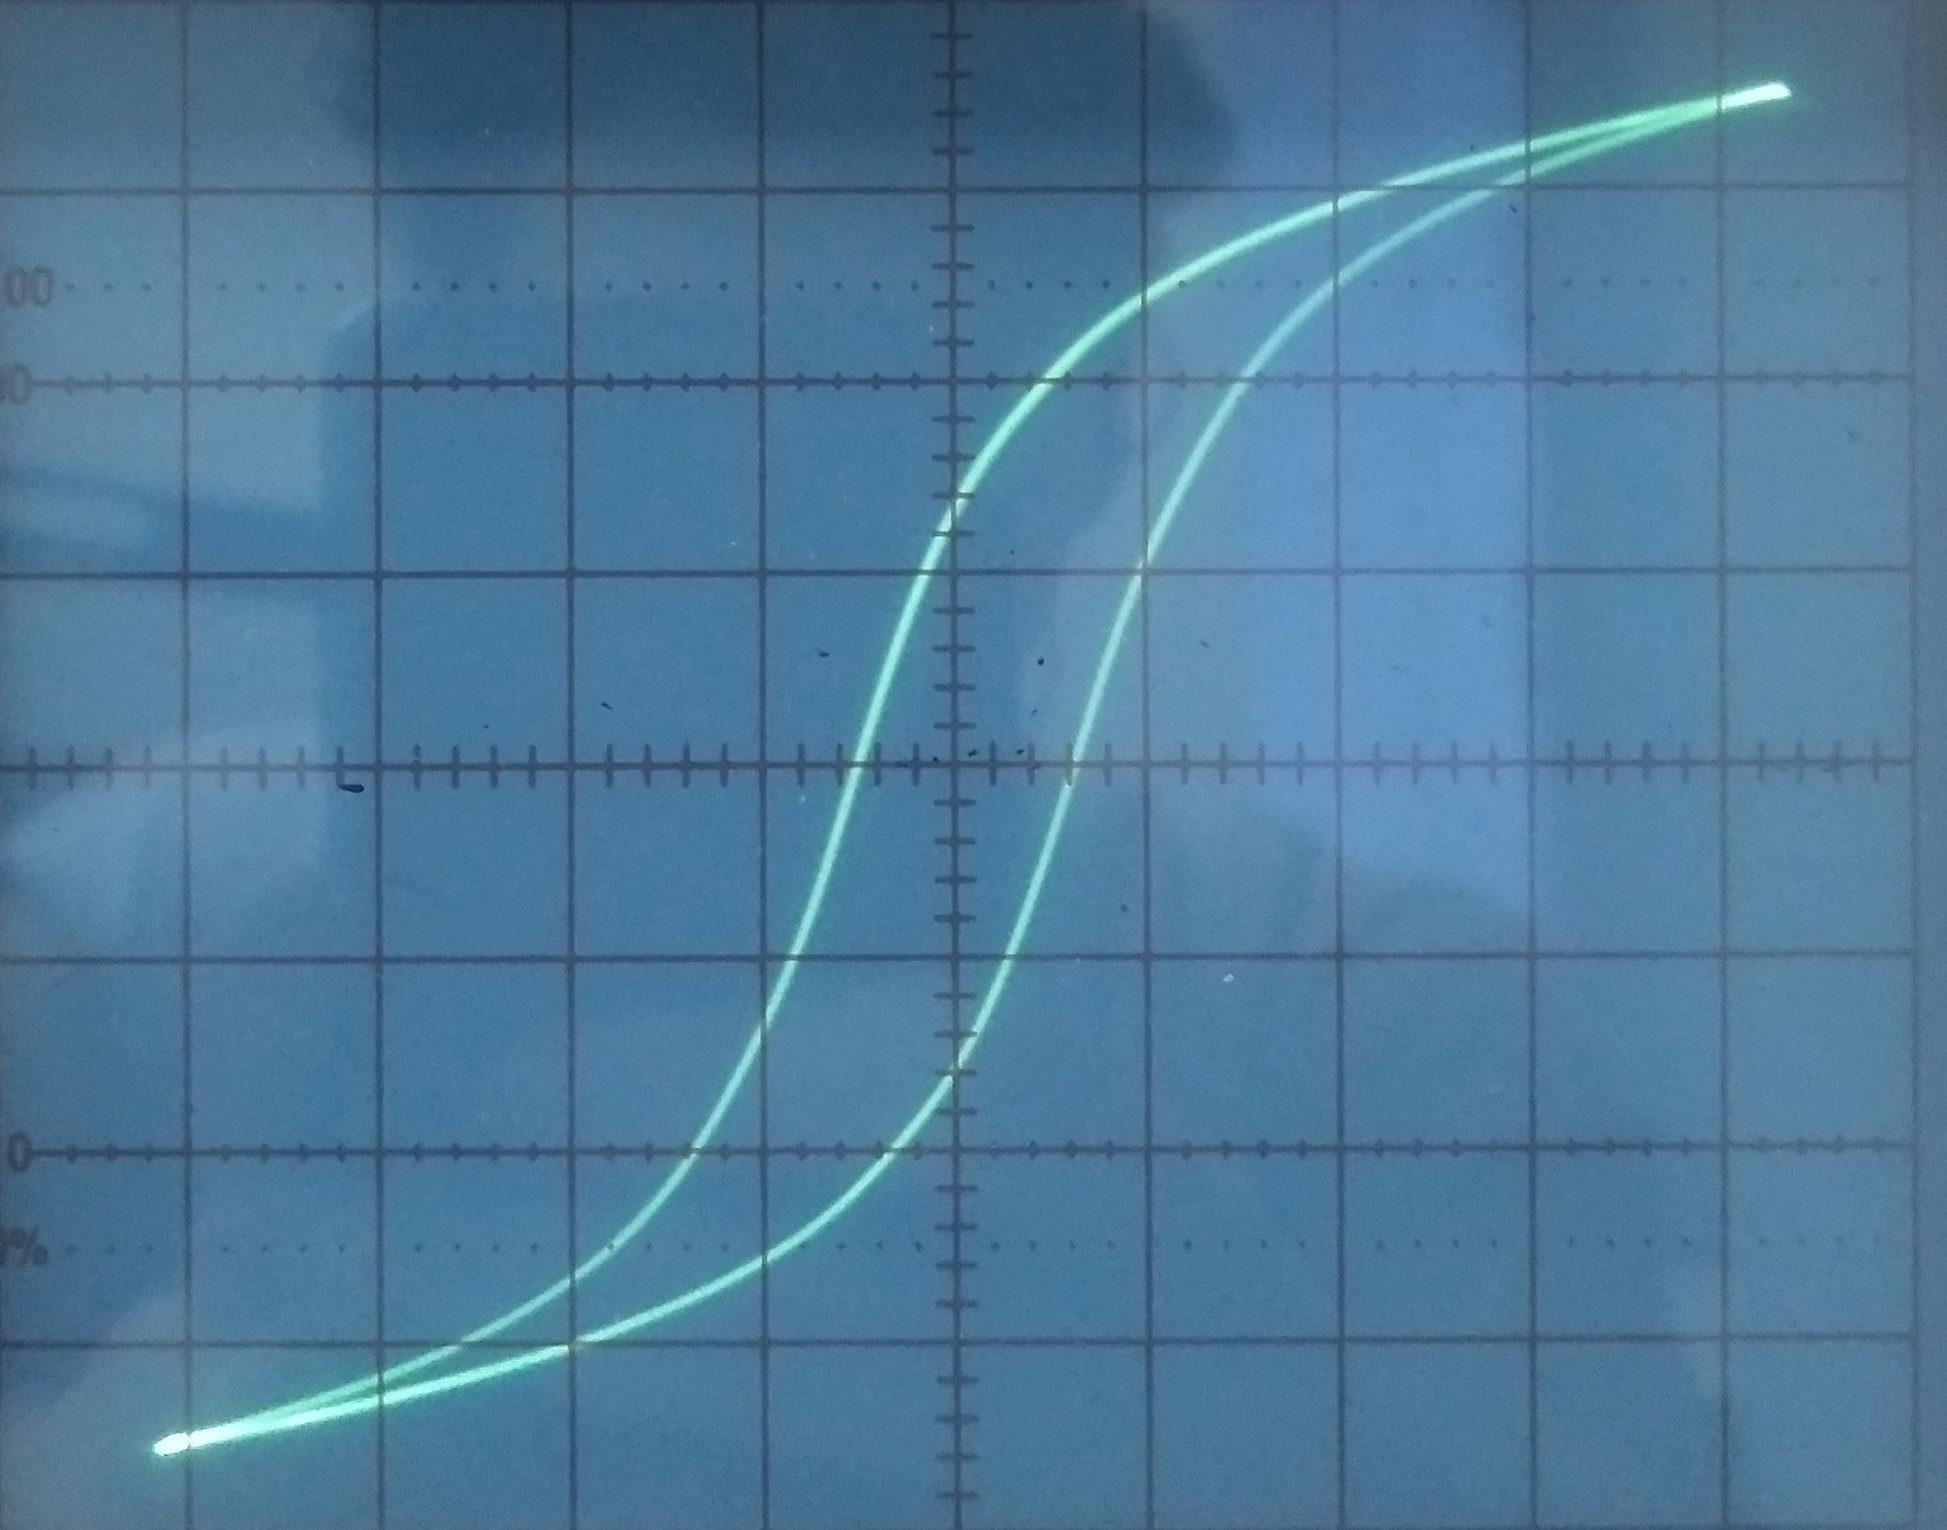
\includegraphics[scale=0.1]{kr1.jpg}
\caption{Максимальная петля гистерезиса для кремниестого железа}
\end{figure}
\begin{figure}[H]
\center
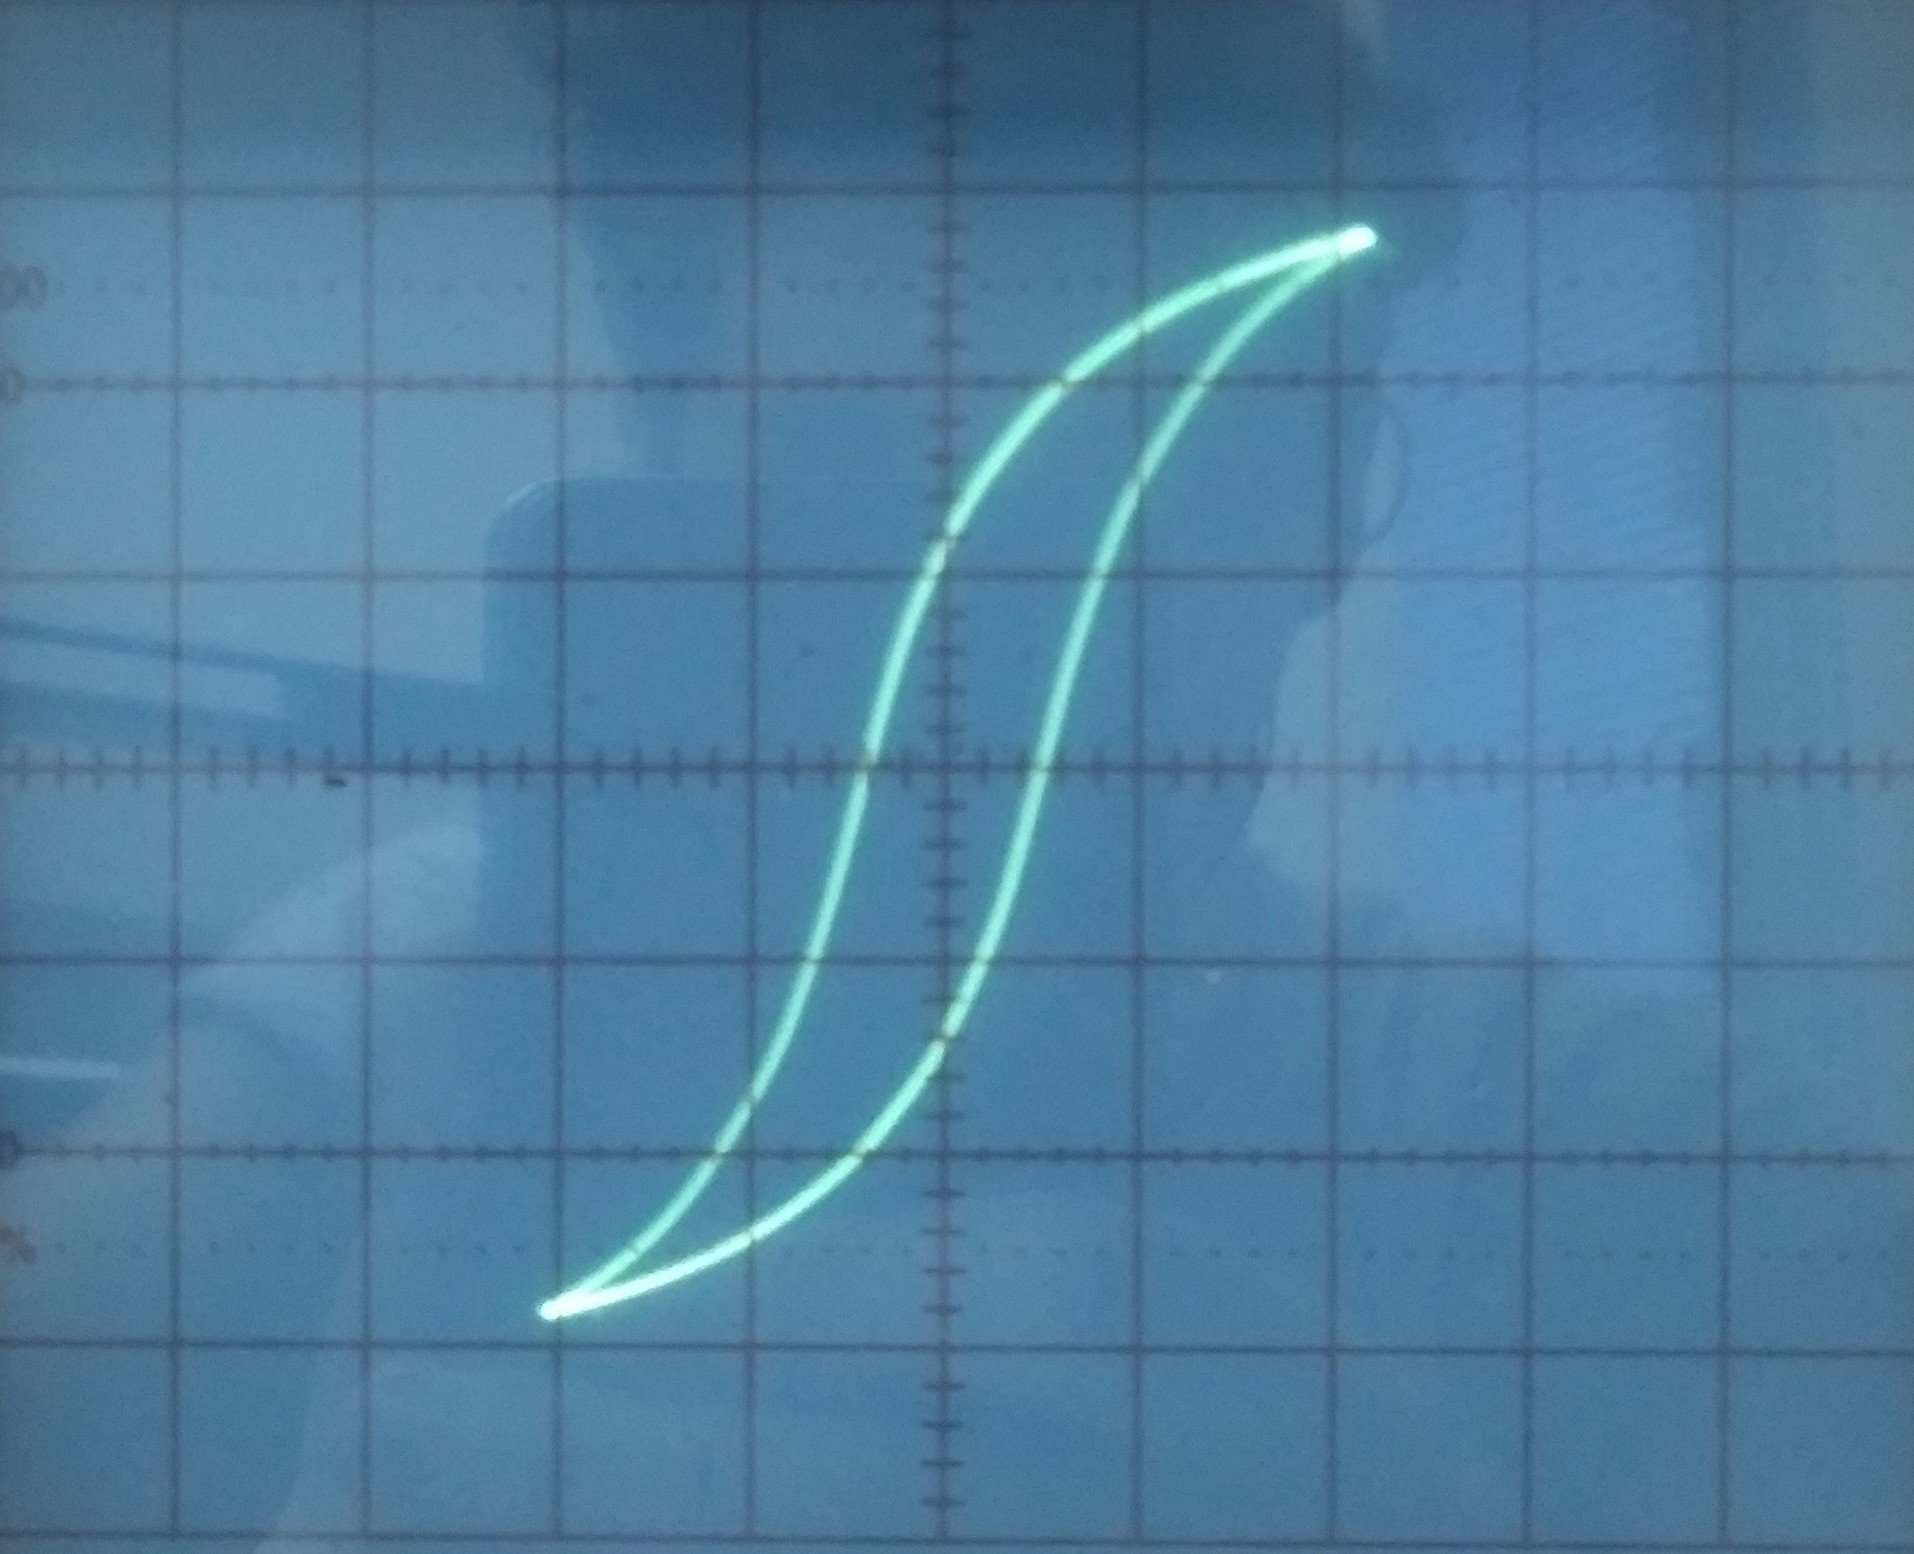
\includegraphics[scale=0.1]{kr2.jpg}
\caption{Петля гистерезиса меньшего размера для кремниестого железа}
\end{figure}

\[
	K_X = 1\ B;\ K_Y = 50\ \text{мВ};\ I_\text{ЭФ} = 0.298 A
\]
\[
	2x(c) = 8.3\ \text{дел};\ 2y(s) = 6.7\ \text{дел}
\]
\[
	H = \frac{I N_0}{2 \pi R} = 113.64\ \frac{A}{\text{м}};\ H_c = 4.5\ \frac{A}{\text{м}}
\]
\[
B = \frac{R_\text{И} C_\text{И} U_\text{ВЫХ}}{S N_\text{И}} = 0.4\ \text{Тл};\ B_s = 1.1\ \text{Тл}
\]
\begin{figure}[H]
\center
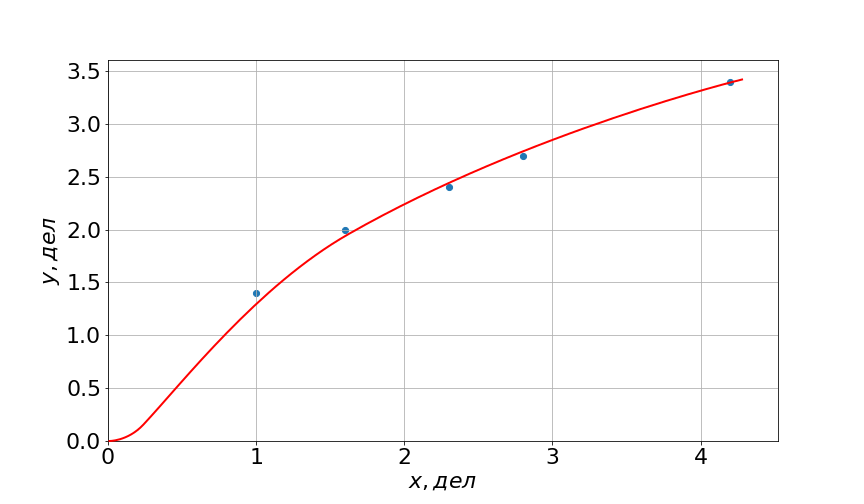
\includegraphics[scale=0.4]{22.png}

\end{figure}


\textbf{Феррит}
\[
	N_0 = 42\ \text{в.};\ N_\text{И} = 400\ \text{в.};\ S = 3.00\ \text{см}^2;\ 2 \pi R = 25.0\ \text{см}
\]
\begin{table}[H]
	\centering
	\begin{tabular}{|c|c|c|} \hline
		$I,\ A$ &  $x,\ \text{дел}$ & $y,\ \text{дел}$ \\\hline
		0.297 & -4.1 & -2.5 \\\hline
		0.248 & -3.5 & -2.3 \\\hline
		0.219 & -3.0 & -2.1 \\\hline
		0.191 & -2.7 & -2.0 \\\hline
		0.166 & -2.3 & -1.7 \\\hline
		0.068 & -1.0 & -0.8 \\\hline
	\end{tabular}	
\end{table}

\begin{figure}[H]
\center
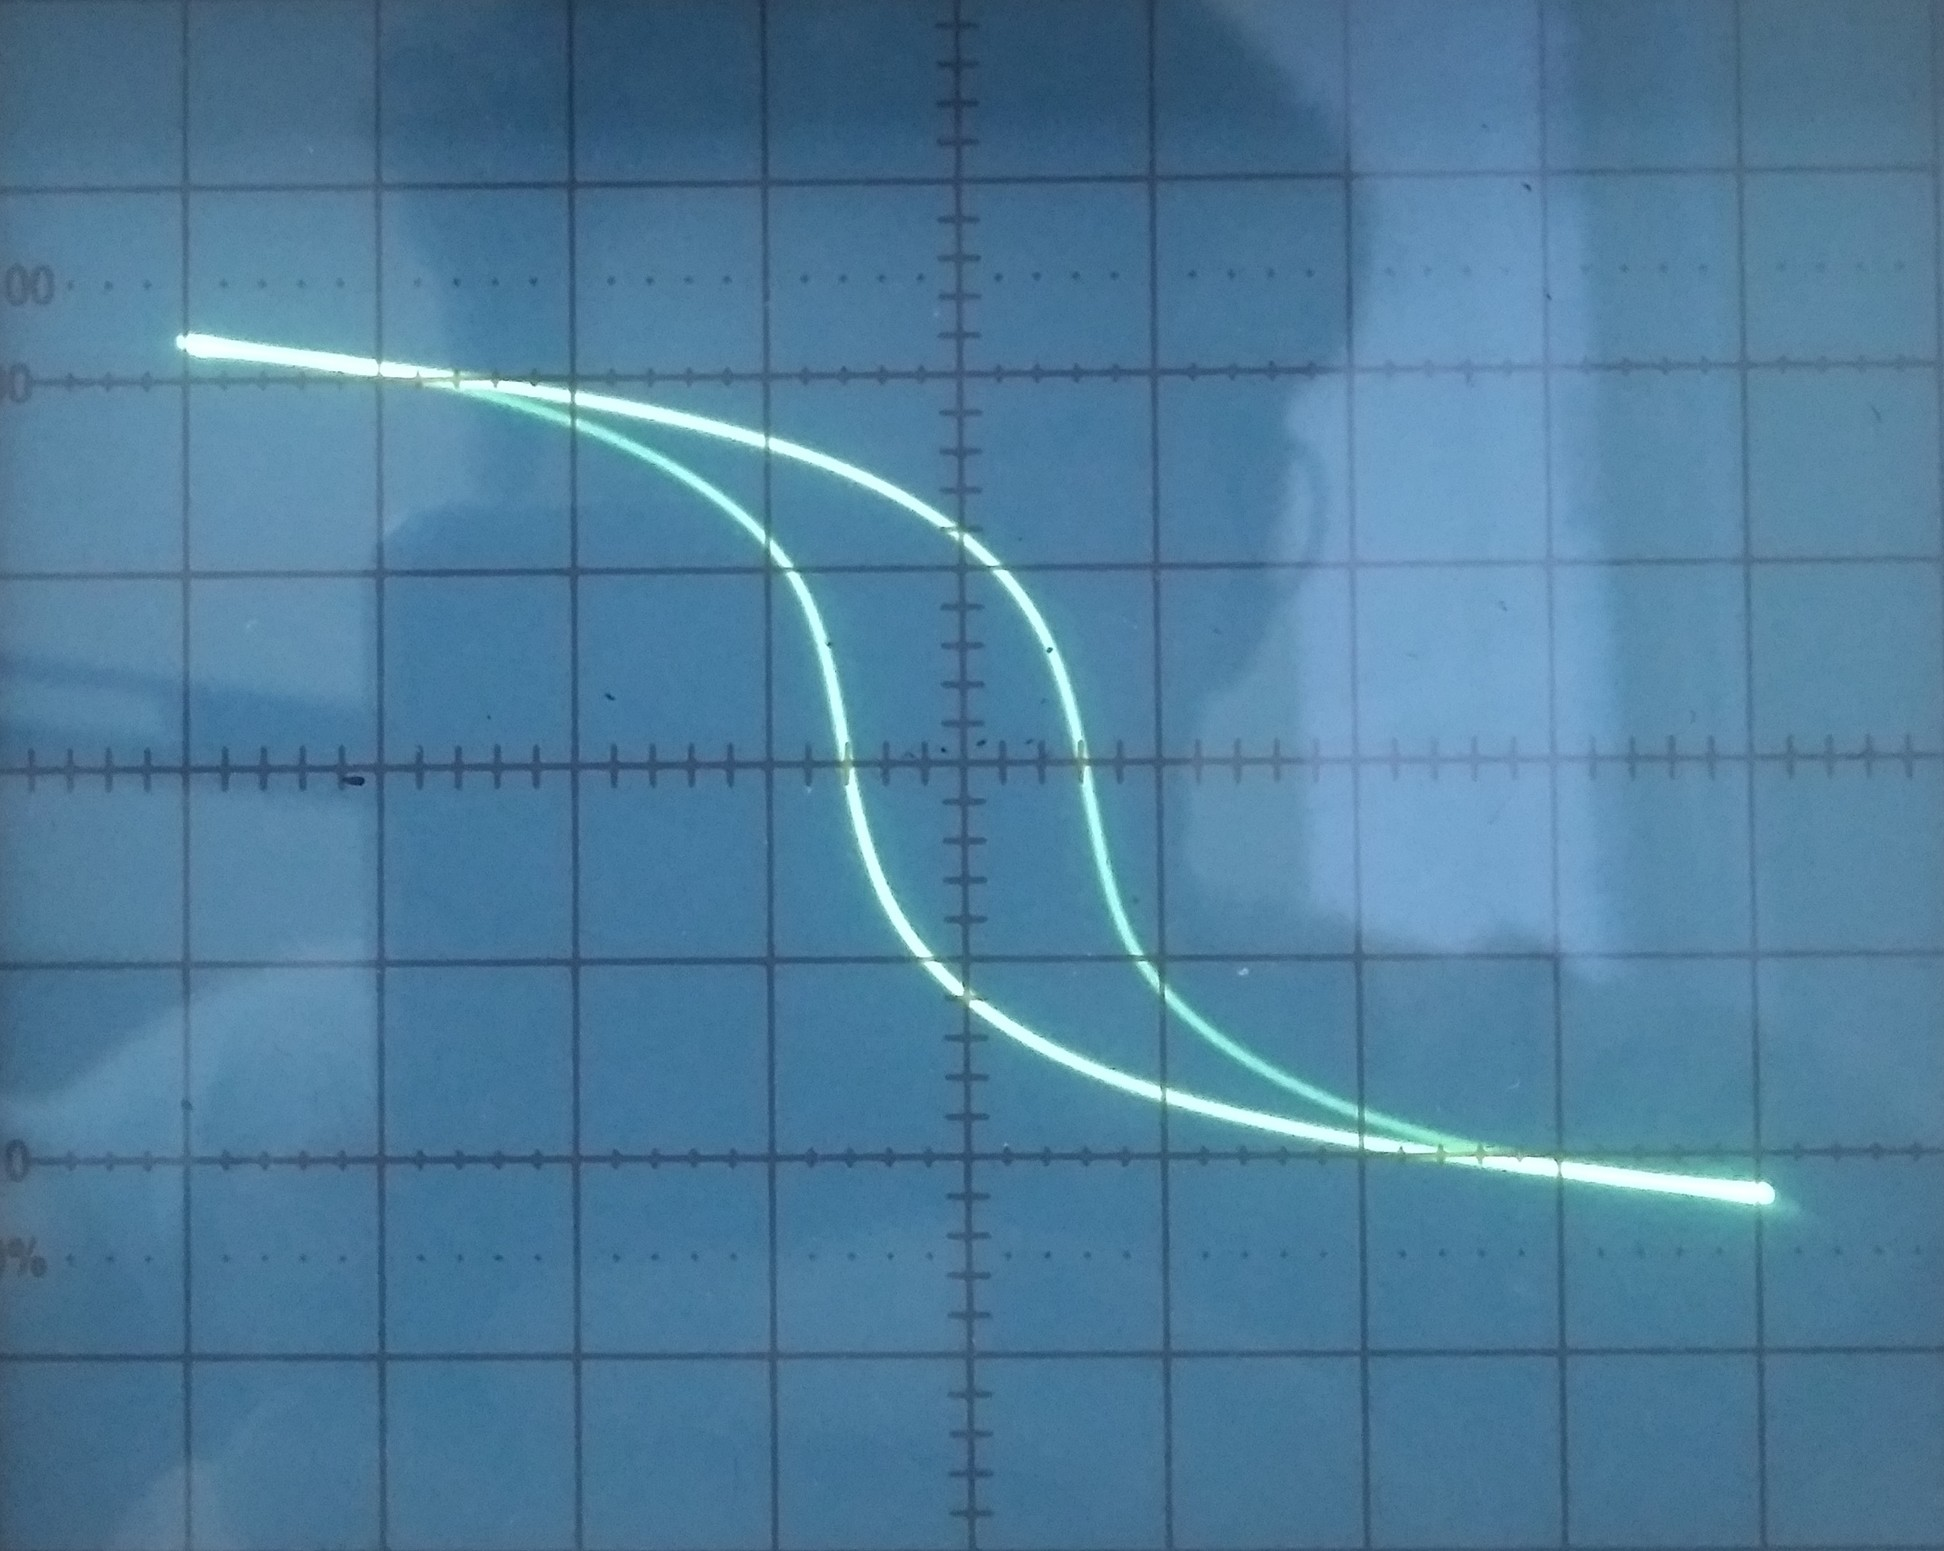
\includegraphics[scale=0.1]{fer.jpg}
\caption{Петля гистерезиса для феррита}
\end{figure}

\[
	K_X = 1\ B;\ K_Y = 50\ \text{мВ};\ I_\text{ЭФ} = 0.298 A
\]
\[
	2x(c) = 8.3\ \text{дел};\ 2y(s) = 6.7\ \text{дел}
\]
\[
	H = \frac{I N_0}{2 \pi R} = 113.64\ \frac{A}{\text{м}};\ H_c = 4.5\ \frac{A}{\text{м}}
\]
\[
B = \frac{R_\text{И} C_\text{И} U_\text{ВЫХ}}{S N_\text{И}} = 0.4\ \text{Тл};\ B_s = 1.1\ \text{Тл}
\]
\begin{figure}[H]
\center
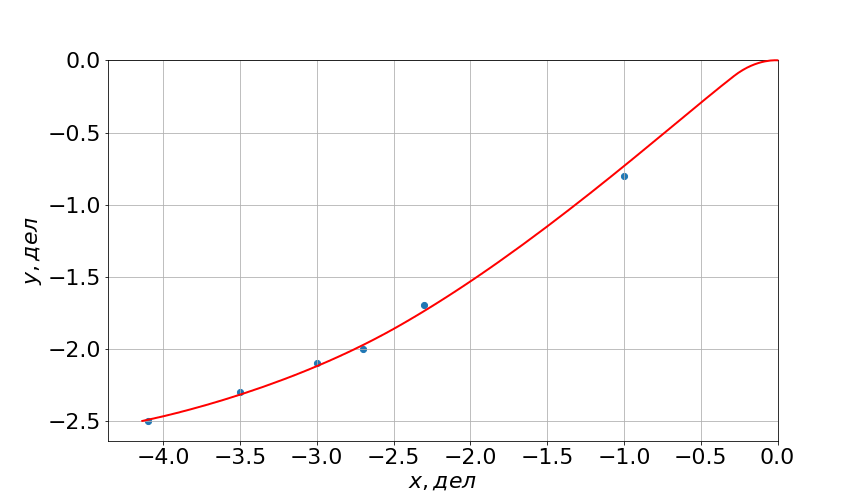
\includegraphics[scale=0.4]{33.png}

\end{figure}
\section*{Вывод}
Петля гистерезиса является качественной характеристикой намагничивания ферромагнетика, показывая такие эффекты, как домены, скачки Баркгаузена (которые можно было бы увидеть при значительно большем масштабе, но в любом случае), в том числе площадь петли пропорциональна энергии, теряемой в единице объёма вещества за время цикла.
\end{document}